% Options for packages loaded elsewhere
\PassOptionsToPackage{unicode}{hyperref}
\PassOptionsToPackage{hyphens}{url}
%
\documentclass[
]{article}
\usepackage{lmodern}
\usepackage{amssymb,amsmath}
\usepackage{ifxetex,ifluatex}
\ifnum 0\ifxetex 1\fi\ifluatex 1\fi=0 % if pdftex
  \usepackage[T1]{fontenc}
  \usepackage[utf8]{inputenc}
  \usepackage{textcomp} % provide euro and other symbols
\else % if luatex or xetex
  \usepackage{unicode-math}
  \defaultfontfeatures{Scale=MatchLowercase}
  \defaultfontfeatures[\rmfamily]{Ligatures=TeX,Scale=1}
\fi
% Use upquote if available, for straight quotes in verbatim environments
\IfFileExists{upquote.sty}{\usepackage{upquote}}{}
\IfFileExists{microtype.sty}{% use microtype if available
  \usepackage[]{microtype}
  \UseMicrotypeSet[protrusion]{basicmath} % disable protrusion for tt fonts
}{}
\makeatletter
\@ifundefined{KOMAClassName}{% if non-KOMA class
  \IfFileExists{parskip.sty}{%
    \usepackage{parskip}
  }{% else
    \setlength{\parindent}{0pt}
    \setlength{\parskip}{6pt plus 2pt minus 1pt}}
}{% if KOMA class
  \KOMAoptions{parskip=half}}
\makeatother
\usepackage{xcolor}
\IfFileExists{xurl.sty}{\usepackage{xurl}}{} % add URL line breaks if available
\IfFileExists{bookmark.sty}{\usepackage{bookmark}}{\usepackage{hyperref}}
\hypersetup{
  pdftitle={Species \& genus plant classification with NEON hyperspectral data},
  pdfauthor={Victoria Scholl; Maxwell B. Joseph},
  pdfkeywords={keyword 1; keyword 2; keyword 3},
  hidelinks,
  pdfcreator={LaTeX via pandoc}}
\urlstyle{same} % disable monospaced font for URLs
\usepackage[margin=1in]{geometry}
\usepackage{longtable,booktabs}
% Correct order of tables after \paragraph or \subparagraph
\usepackage{etoolbox}
\makeatletter
\patchcmd\longtable{\par}{\if@noskipsec\mbox{}\fi\par}{}{}
\makeatother
% Allow footnotes in longtable head/foot
\IfFileExists{footnotehyper.sty}{\usepackage{footnotehyper}}{\usepackage{footnote}}
\makesavenoteenv{longtable}
\usepackage{graphicx,grffile}
\makeatletter
\def\maxwidth{\ifdim\Gin@nat@width>\linewidth\linewidth\else\Gin@nat@width\fi}
\def\maxheight{\ifdim\Gin@nat@height>\textheight\textheight\else\Gin@nat@height\fi}
\makeatother
% Scale images if necessary, so that they will not overflow the page
% margins by default, and it is still possible to overwrite the defaults
% using explicit options in \includegraphics[width, height, ...]{}
\setkeys{Gin}{width=\maxwidth,height=\maxheight,keepaspectratio}
% Set default figure placement to htbp
\makeatletter
\def\fps@figure{htbp}
\makeatother
\setlength{\emergencystretch}{3em} % prevent overfull lines
\providecommand{\tightlist}{%
  \setlength{\itemsep}{0pt}\setlength{\parskip}{0pt}}
\setcounter{secnumdepth}{5}
% clean citations
\usepackage{natbib}
\bibliographystyle{ecology}
\setcitestyle{authoryear,open={(},close={)}}

% line numbers
\usepackage[left]{lineno}

\usepackage[margin=1in]{geometry}

% prevent hyphenated wrap
\usepackage[none]{hyphenat}

% bold math for matrices
% https://tex.stackexchange.com/questions/199789/which-bold-style-is-recommended-for-matrix-notation
\newcommand{\matr}[1]{\mathbf{#1}}

% block arrays for matrices with labeled rows and columns
\usepackage{blkarray}

% monospace font for inline code
\def\code#1{\texttt{#1}}

% easy equation alignment
\usepackage{amsmath}

\usepackage{setspace}
\doublespacing

\title{Species \& genus plant classification with NEON hyperspectral data}
\author{Victoria Scholl\thanks{victoria.scholl@colorado.edu, Earth Lab and Geography Dept., University of Colorado, Boulder, CO 80303, USA} \and Maxwell B. Joseph\thanks{maxwell.b.joseph@colorado.edu, Earth Lab, University of Colorado, Boulder, CO 80303, USA}}
\date{}

\begin{document}
\maketitle
\begin{abstract}
Text of abstract
\end{abstract}

Keywords: keyword 1; keyword 2; keyword 3

Highlights: These are the highlights.

\hypertarget{introduction}{%
\section{Introduction}\label{introduction}}

The National Ecological Observatory Network (NEON) is a valuable source of publicly available ecological data across the United States (Keller et al. 2008).

We have extracted all NEON AOP hyperspectral data for every mapped stem in NEON plots where field data and airborne remote sensing data were collected during the same year.

Here's the code to extract the spectra: \url{https://gist.github.com/mbjoseph/5c18781e508460e14f64193571b98b7d}

We used a machine learning approach to evaluate plant identification potential using the hyperspectral data at multiple taxonomic resolutions: species and genus levels.

Species classification is an active research area (Scholl et al. 2020).

\hypertarget{background}{%
\section{Background}\label{background}}

\hypertarget{methods}{%
\section{Methods}\label{methods}}

\hypertarget{data-cleaning}{%
\subsection{Data cleaning}\label{data-cleaning}}

\hypertarget{species-classification}{%
\subsection{Species classification}\label{species-classification}}

\hypertarget{genus-classification}{%
\subsection{Genus classification}\label{genus-classification}}

Same setup as species classification, but used the genus as each class label.

\hypertarget{results}{%
\section{Results}\label{results}}

\begin{figure}
\centering
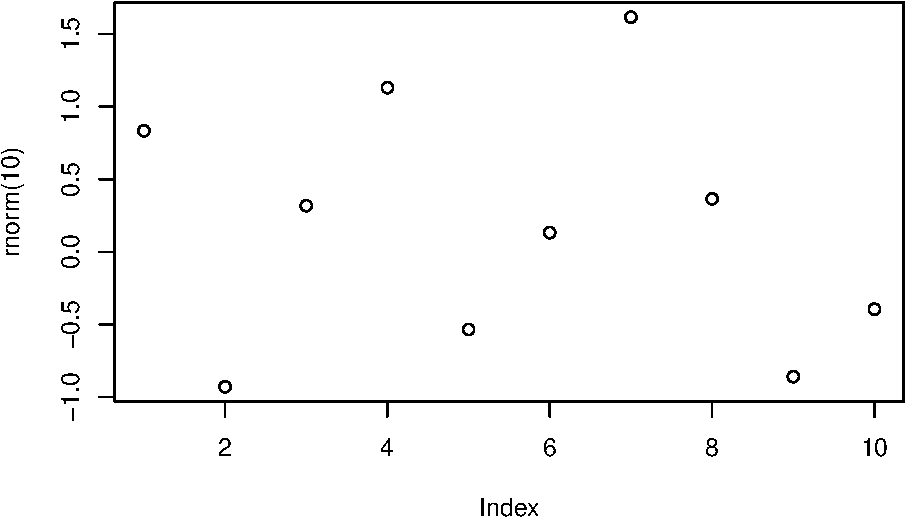
\includegraphics{../figures/demo-plot-1.pdf}
\caption{\label{fig:demo-plot}A plot of random numbers}
\end{figure}

Figure \ref{fig:demo-plot} shows how we can have a caption and cross-reference for a plot

Here is an example of inline code 3.14 in the middle of a sentence.

\hypertarget{discussion}{%
\section{Discussion}\label{discussion}}

\hypertarget{conclusion}{%
\section{Conclusion}\label{conclusion}}

\hypertarget{acknowledgements}{%
\section{Acknowledgements}\label{acknowledgements}}

Max has cool ideas and knows many R tricks

\newpage

\hypertarget{references}{%
\section{References}\label{references}}

\hypertarget{refs}{}
\leavevmode\hypertarget{ref-keller2008continental}{}%
Keller, M., D. S. Schimel, W. W. Hargrove, and F. M. Hoffman. 2008. A continental strategy for the national ecological observatory network. The Ecological Society of America: 282-284.

\leavevmode\hypertarget{ref-scholl2020integrating}{}%
Scholl, V. M., M. E. Cattau, M. B. Joseph, and J. K. Balch. 2020. Integrating national ecological observatory network (neon) airborne remote sensing and in-situ data for optimal tree species classification. Remote Sensing 12:1414.

\newpage

\clearpage

\hypertarget{figure-legends}{%
\section*{Figure legends}\label{figure-legends}}
\addcontentsline{toc}{section}{Figure legends}

\hypertarget{figure-1}{%
\subsection*{Figure 1}\label{figure-1}}
\addcontentsline{toc}{subsection}{Figure 1}

Figure 1 info\ldots{}

\hypertarget{figure-2}{%
\subsection*{Figure 2}\label{figure-2}}
\addcontentsline{toc}{subsection}{Figure 2}

It ain't much\ldots{}

\hypertarget{figures}{%
\section*{Figures}\label{figures}}
\addcontentsline{toc}{section}{Figures}

\hypertarget{figure-1-1}{%
\subsection*{Figure 1}\label{figure-1-1}}
\addcontentsline{toc}{subsection}{Figure 1}

\begin{figure}
\includegraphics[width=450px]{/Users/victoriascholl/github/neonHScompendium/analysis/figures/spectra_figure_test} \end{figure}

\clearpage

\hypertarget{figure-2-1}{%
\subsection*{Figure 2}\label{figure-2-1}}
\addcontentsline{toc}{subsection}{Figure 2}

\begin{figure}
\includegraphics[width=450px]{/Users/victoriascholl/github/neonHScompendium/analysis/figures/honest_work} \end{figure}

\clearpage

\end{document}
